% LaTeX Source
%
% Author:        Filipe L B Correia <filipelbc@gmail.com>
% Last Change:   2015 Out 11 15:11:15

\documentclass{rosario}

%===============================================================================
\begin{document}

\title{O Santo\\Rosário}
\author{}
\date{}

\maketitle

%===============================================================================

\chapter{Instruções}

\begin{center}
    
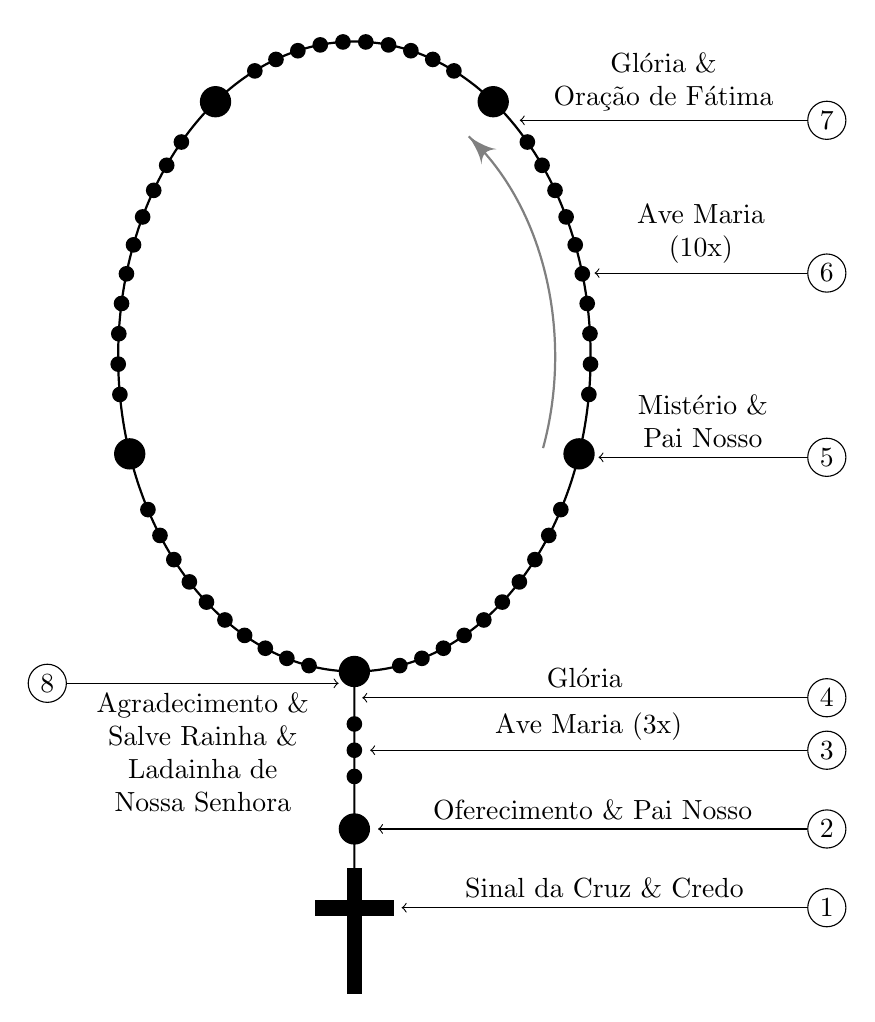
\begin{tikzpicture}[x=1mm,y=1mm]

    
\newcommand{\lx}{30}
\newcommand{\ly}{40}
\newcommand{\ld}{20}
\newcommand{\lw}{1}
\newcommand{\lp}{(2*\lx)}

\tikzstyle{conta}=[circle,fill,inner sep=2]
\tikzstyle{misterio}=[circle,fill,inner sep=4]

\draw[thick] (0,0) ellipse ({\lx} and {\ly}) (0,{-\ly}) -- ++(0,{-\ld}) node[misterio] {} -- ++(0,{-\ld/4});

\fill[] ({-\lw},{-\ly-5*\ld/4}) rectangle ++({2*\lw},{-16*\lw});
\fill[] ({-5*\lw},{-\ly-5*\ld/4-4*\lw}) rectangle ++({10*\lw},{-2*\lw});

\foreach \d in {0,1,2}
{
    \path (0,{-\ly}) ++(0,{-(\d + 2)*\ld/6}) node[conta] {};
}

\foreach \a in {-90,-18,...,198}
{
    \path (0,0) + ({\lx},0) arc (0:{\a}:{\lx} and {\ly}) node[misterio] {};

    \foreach \b in {0,...,9}
    {
        \path (0,0) + ({\lx},0) arc (0:{\a+(\b+2)*72/13}:{\lx} and {\ly}) node[conta] {};
    }
}


    \usetikzlibrary{arrows,decorations.markings}

    \tikzstyle{passo}=[circle,draw,inner sep=2]
    \tikzstyle{seta}=[decoration={markings,mark=at position 1 with
                        {\arrow[scale=2,>=latex']{>}}},postaction={decorate}]

    \newcommand{\indique}[5]{
        \node[passo] (#1) at ({\lp},{#3}) {$#5$};
        \draw[<-] ({#4},{#3}) -- node[anchor=south,align=center] {#2} (#1);
    }

    \newcommand{\sentido}[3]{
        \draw[gray,seta,thick] ({#1*cos(#2)*\lx},{#1*sin(#2)*\ly}) arc ({#2}:{#3}:{#1*\lx} and {#1*\ly}) --++ (-0.1,0.1);
    }

    \sentido{0.85}{-20}{55}

    \indique{credo}{Sinal da Cruz \& Credo}{-\ly-5*\ld/4-5*\lw}{6*\lw}{1}

    \indique{painosso}{Oferecimento \& Pai Nosso}{-\ly-\ld}{3}{2}

    \indique{avemaria}{Ave Maria (3x)}{-\ly-\ld/2}{2}{3}

    \indique{gloria}{Glória}{-\ly-\ld/6}{1}{4}

    \indique{anuncio2}{Mistério \&\\ Pai Nosso}{-0.32*\ly}{\lx+\lw}{5}

    \indique{avemaria2}{Ave Maria\\(10x)}{0.265*\ly}{\lx+0.5*\lw}{6}

    \indique{fatima}{Glória \&\\ Oração de Fátima}{0.75*\ly}{0.70*\lx}{7}

    \renewcommand{\indique}[5]{
        \node[passo] (#1) at ({-0.65*\lp},{#3}) {$#5$};
        \draw[->] (#1) -- node[anchor=north,align=center] {#2} ({#4},{#3});
    }

    \indique{salve}{Agradecimento \&\\Salve Rainha \&\\ Ladainha de\\ Nossa Senhora}{-\ly-1.5*\lw}{-2*\lw}{8}

\end{tikzpicture}


\end{center}

\TODO

%===============================================================================

\chapter{Orações}

%===============================================================================

\section{Sinal da Cruz}

Pelo Sinal da santa cruz, livrai-nos Deus Nosso Senhor dos nossos inimigos.

Em nome do Pai, do Filho e do Espírito Santo.

\amen.

%===============================================================================

\section{Credo Apostólico}

Creio em Deus Pai, todo-poderoso, Criador do céu e da terra.

E em Jesus Cristo, seu único Filho, nosso Senhor,
que foi concebido pelo poder do Espírito Santo;
nasceu da Virgem Maria;
padeceu sob Pôncio Pilatos;
foi crucificado, morto e sepultado;
desceu à mansão dos mortos;
ressuscitou ao terceiro dia;
subiu aos céus;
e está sentado à direita de Deus Pai todo-poderoso,
donde há de vir a julgar os vivos e os mortos.

Creio no Espírito Santo;
na santa Igreja Católica;
na comunhão dos santos;
na remissão dos pecados;
na ressurreição da carne;
na vida eterna.

\amen.

%===============================================================================

\section{Pai Nosso}

Pai nosso, que estais no céu,
santificado seja o vosso nome;
venha a nós o vosso reino;
seja feita a vossa vontade,
assim na terra como no céu;
o pão nosso de cada dia nos dai hoje;
perdoai-nos as nossas dívidas,
assim como nós perdoamos aos nossos devedores;
e não nos deixeis cair em tentação;
mas livrai-nos do mal.

\amen.

%===============================================================================

\section{Ave Maria}

Ave, Maria, cheia de graça,
o Senhor é convosco;
bendita sois vós entre as mulheres,
e bendito é o fruto do vosso ventre,
Jesus.

Santa Maria, Mãe de Deus,
rogai por nós, pecadores,
agora e na hora da nossa morte.

\amen.

%===============================================================================

\section{Salve Rainha}

Salve, Rainha,
Mãe de misericórdia,
vida, doçura e esperança nossa, salve!
A vós bradamos, os degredados filhos de Eva;
a vós suspiramos, gemendo e chorando neste vale de lágrimas.
Eia pois, advogada nossa,
esses vossos olhos misericordiosos a nós volvei;
e no fim deste desterro nos mostrai Jesus,
bendito fruto do vosso ventre,
ó clemente, ó piedosa, ó doce sempre Virgem Maria.

Rogai por nós, santa Mãe de Deus. \\
Para que sejamos dignos das promessas de Cristo.

%===============================================================================

\section{Glória}

Glória ao Pai, ao Filho, e ao Espírito Santo. \\
Como era no princípio, agora e sempre.

\amen.

%===============================================================================

\section{Oração de Fátima}

Ó meu bom Jesus!
Perdoai-nos;
livrai-nos do fogo do inferno;
levai as almas para o céu
e socorrei principalmente as que mais precisarem.

\amen.

%===============================================================================

\chapter{Mistérios Gozosos}

\emph{Segundas e Sábados.}

\from{RVM 20:}

[Estes mistérios] caracteriza[m]-se de facto pela \emph{alegria que irradia do acontecimento da Encarnação}.
Isto é evidente desde a Anunciação, quando a saudação de Gabriel à Virgem de Nazaré se liga ao convite da alegria messiânica:
<< Alegra-te, Maria >>.
Para este anúncio se encaminha a história da salvação, e até, de certo modo, a história do mundo.
De facto, se o desígnio do Pai é recapitular em Cristo todas as coisas (cf. Ef 1, 10), então todo o
universo de algum modo é alcançado pelo favor divino, com o qual o Pai Se inclina sobre Maria
para torná-La Mãe do seu Filho.
Por sua vez, toda a humanidade está como que incluída no fiat com que Ela corresponde prontamente à vontade de Deus.

Sob o signo da exultação, aparece depois a cena do encontro com Isabel, onde a mesma voz de Maria e a presença de Cristo no seu ventre fazem << saltar de alegria >> João (cf. Lc 1, 44).
Inundada de alegria é a cena de Belém, onde o nascimento do Deus-Menino, o Salvador do mundo, é cantado pelos anjos e anunciado aos pastores precisamente como << uma grande alegria >> (Lc 2, 10).

Os dois últimos mistérios, porém, mesmo conservando o sabor da alegria \emph{antecipam já os sinais do drama}.
A apresentação no templo, de facto, enquanto exprime a alegria da consagração e extasia o velho Simeão, regista também a profecia do << sinal de contradição >> que o Menino será para Israel e da espada que trespassará a alma da Mãe (cf. Lc 2, 34-35).
Gozoso e ao mesmo tempo dramático é também o episódio de Jesus, aos doze anos, no templo.
Vemo-Lo aqui na sua divina sabedoria, enquanto escuta e interroga, e substancialmente no papel d'Aquele que ``ensina''.
A revelação do seu mistério de Filho totalmente dedicado às coisas do Pai é anúncio daquela radicalidade evangélica que põe inclusive em crise os laços mais caros do homem, diante das exigências absolutas do Reino.
Até José e Maria, aflitos e angustiados, << não entenderam >> as suas palavras (Lc 2, 50).

Por isso, meditar os mistérios gozosos significa entrar nas motivações últimas e no significado profundo da alegria cristã.
Significa fixar o olhar sobre a realidade concreta do mistério da Encarnação e sobre o obscuro prenúncio do mistério do sofrimento salvífico.
Maria leva-nos a aprender o segredo da alegria cristã, lembrando-nos que o cristianismo é, antes de mais, \emph{euangelion}, ``boa nova'', que tem o seu centro, antes, o seu mesmo conteúdo, na pessoa de Cristo, o Verbo feito carne, único Salvador do mundo.

%===============================================================================

\section{A Anunciação do Anjo a Nossa Senhora}

\from{Mateus \TODO:}

\from{Marcos \TODO:}

\from{Lucas 1, 26--39:}

No sexto mês, o anjo Gabriel foi enviado por Deus a uma cidade da Galiléia, chamada Nazaré,
a uma virgem desposada com um homem que se chamava José, da casa de Davi e o nome da virgem era Maria.
Entrando, o anjo disse-lhe:
Ave, cheia de graça, o Senhor é contigo.
Perturbou-se ela com estas palavras e pôs-se a pensar no que significaria semelhante saudação.
O anjo disse-lhe:
Não temas, Maria, pois encontraste graça diante de Deus.
Eis que conceberás e darás à luz um filho, e lhe porás o nome de Jesus.
Ele será grande e chamar-se-á Filho do Altíssimo, e o Senhor Deus lhe dará o trono de seu pai Davi;
e reinará eternamente na casa de Jacó,
e o seu reino não terá fim.
Maria perguntou ao anjo:
Como se fará isso, pois não conheço homem?
Respondeu-lhe o anjo:
O Espírito Santo descerá sobre ti, e a força do Altíssimo te envolverá com a sua sombra.
Por isso o ente santo que nascer de ti será chamado Filho de Deus.
Também Isabel, tua parenta, até ela concebeu um filho na sua velhice;
e já está no sexto mês aquela que é tida por estéril,
porque a Deus nenhuma coisa é impossível.
Então disse Maria:
Eis aqui a serva do Senhor.
Faça-se em mim segundo a tua palavra.
E o anjo afastou-se dela.

\from{João \TODO:}

\from{CIC 484:}

A Anunciação a Maria inaugura a << plenitude dos tempos >> (Gl 4, 4), isto é, o cumprimento das promessas e dos preparativos.
Maria é convidada a conceber Aquele em quem habitará << corporalmente toda a plenitude da Divindade >> (Cl 2, 9).
A resposta divina ao seu << como será isto, se Eu não conheço homem? >> (Lc 1, 34) é dada pelo poder do Espírito:
<< O Espírito Santo virá sobre ti >> (Lc 1, 35).

%===============================================================================

\section{A Visitação de Nossa Senhora a Santa Isabel}

\from{Mateus \TODO:}

\from{Marcos \TODO:}

\from{Lucas 1, 39--56:}

Naqueles dias, Maria se levantou e foi às pressas às montanhas, a uma cidade de Judá.
Entrou em casa de Zacarias e saudou Isabel.
Ora, apenas Isabel ouviu a saudação de Maria, a criança estremeceu no seu seio;
e Isabel ficou cheia do Espírito Santo.
E exclamou em alta voz:
Bendita és tu entre as mulheres e bendito é o fruto do teu ventre.
Donde me vem esta honra de vir a mim a mãe de meu Senhor?
Pois assim que a voz de tua saudação chegou aos meus ouvidos, a criança estremeceu de alegria no meu seio.
Bem-aventurada és tu que creste, pois se hão de cumprir as coisas que da parte do Senhor te foram ditas!
E Maria disse:
Minha alma glorifica ao Senhor,
meu espírito exulta de alegria em Deus, meu Salvador,
porque olhou para sua pobre serva.
Por isto, desde agora, me proclamarão bem-aventurada todas as gerações,
porque realizou em mim maravilhas aquele que é poderoso e cujo nome é Santo.
Sua misericórdia se estende, de geração em geração, sobre os que o temem.
Manifestou o poder do seu braço:
desconcertou os corações dos soberbos.
Derrubou do trono os poderosos e exaltou os humildes.
Saciou de bens os indigentes e despediu de mãos vazias os ricos.
Acolheu a Israel, seu servo, lembrado da sua misericórdia,
conforme prometera a nossos pais, em favor de Abraão e sua posteridade, para sempre.
Maria ficou com Isabel cerca de três meses.
Depois voltou para casa.

\from{João \TODO:}

\from{CIC 717:}

<< Apareceu um homem, enviado por Deus, que tinha o nome de João >> (Jo 1, 6).
João é << cheio do Espírito Santo já desde o seio materno >> (Lc 1, 15), pelo próprio Cristo que a Virgem acabava de conceber por obra e graça do Espírito Santo.
A << visitação >> de Maria a Isabel tornou-se, assim, << visita de Deus ao seu povo >>.

%===============================================================================

\section{O Nascimento do Menino Jesus em Belém}

\from{Mateus 2, 1--16:}

\TODO

\from{Marcos \TODO:}

\from{Lucas 2, 1--20:}

Naqueles tempos apareceu um decreto de César Augusto, ordenando o recenseamento de toda a terra.
Este recenseamento foi feito antes do governo de Quirino, na Síria.
Todos iam alistar-se, cada um na sua cidade.
Também José subiu da Galiléia, da cidade de Nazaré, à Judéia, à Cidade de Davi, chamada Belém, porque era da casa e família de Davi,
para se alistar com a sua esposa Maria, que estava grávida.
Estando eles ali, completaram-se os dias dela.
E deu à luz seu filho primogênito, e, envolvendo-o em faixas, reclinou-o num presépio;
porque não havia lugar para eles na hospedaria.
Havia nos arredores uns pastores, que vigiavam e guardavam seu rebanho nos campos durante as vigílias da noite.
Um anjo do Senhor apareceu-lhes e a glória do Senhor refulgiu ao redor deles, e tiveram grande temor.
O anjo disse-lhes:
Não temais, eis que vos anuncio uma boa nova que será alegria para todo o povo:
hoje vos nasceu na Cidade de Davi um Salvador, que é o Cristo Senhor.
Isto vos servirá de sinal:
achareis um recém-nascido envolto em faixas e posto numa manjedoura.
E subitamente ao anjo se juntou uma multidão do exército celeste, que louvava a Deus e dizia:
Glória a Deus no mais alto dos céus e na terra paz aos homens, objetos da benevolência (divina).
Depois que os anjos os deixaram e voltaram para o céu, falaram os pastores uns com os outros:
Vamos até Belém e vejamos o que se realizou e o que o Senhor nos manifestou.
Foram com grande pressa e acharam Maria e José, e o menino deitado na manjedoura.
Vendo-o, contaram o que se lhes havia dito a respeito deste menino.
Todos os que os ouviam admiravam-se das coisas que lhes contavam os pastores.
Maria conservava todas estas palavras, meditando-as no seu coração.
Voltaram os pastores, glorificando e louvando a Deus por tudo o que tinham ouvido e visto, e que estava de acordo com o que lhes fora dito.

\from{João \TODO:}

\from{CIC 525:}

Jesus nasceu na humildade dum estábulo, no seio duma família pobre.
As primeiras testemunhas deste acontecimento são simples pastores.
E é nesta pobreza que se manifesta a glória do céu.
A Igreja não se cansa de cantar a glória desta noite:

\begin{verse}
Hoje a Virgem dá à luz o Eterno \\
e a terra oferece uma gruta ao Inacessível. \\
Cantam-n'O os anjos e os pastores, \\
e com a estrela os magos põem-se a caminho, \\
porque Tu nasceste para nós, \\
pequeno Infante. Deus eterno!
\end{verse}

%===============================================================================

\section{A Apresentação de Jesus no Templo}

\from{Mateus \TODO:}

\from{Marcos \TODO:}

\from{Lucas 2, 21--40:}

Completados que foram os oito dias para ser circuncidado o menino, foi-lhe posto o nome de Jesus, como lhe tinha chamado o anjo, antes de ser concebido no seio materno.
Concluídos os dias da sua purificação segundo a Lei de Moisés, levaram-no a Jerusalém para o apresentar ao Senhor,
conforme o que está escrito na lei do Senhor:
Todo primogênito do sexo masculino será consagrado ao Senhor (Ex 13,2);
e para oferecerem o sacrifício prescrito pela lei do Senhor, um par de rolas ou dois pombinhos.
Ora, havia em Jerusalém um homem chamado Simeão.
Este homem, justo e piedoso, esperava a consolação de Israel, e o Espírito Santo estava nele.
Fora-lhe revelado pelo Espírito Santo que não morreria sem primeiro ver o Cristo do Senhor.
Impelido pelo Espírito Santo, foi ao templo.
E tendo os pais apresentado o menino Jesus, para cumprirem a respeito dele os preceitos da lei,
tomou-o em seus braços e louvou a Deus nestes termos:
Agora, Senhor, deixai o vosso servo ir em paz, segundo a vossa palavra.
Porque os meus olhos viram a vossa salvação
que preparastes diante de todos os povos,
como luz para iluminar as nações, e para a glória de vosso povo de Israel.
Seu pai e sua mãe estavam admirados das coisas que dele se diziam.
Simeão abençoou-os e disse a Maria, sua mãe:
Eis que este menino está destinado a ser uma causa de queda e de soerguimento para muitos homens em Israel, e a ser um sinal que provocará contradições,
a fim de serem revelados os pensamentos de muitos corações.
E uma espada transpassará a tua alma.
Havia também uma profetisa chamada Ana, filha de Fanuel, da tribo de Aser;
era de idade avançada.
Depois de ter vivido sete anos com seu marido desde a sua virgindade, ficara viúva, e agora com oitenta e quatro anos não se apartava do templo, servindo a Deus noite e dia em jejuns e orações.
Chegando ela à mesma hora, louvava a Deus e falava de Jesus a todos aqueles que em Jerusalém esperavam a libertação.
Após terem observado tudo segundo a lei do Senhor, voltaram para a Galiléia, à sua cidade de Nazaré.
O menino ia crescendo e se fortificava:
estava cheio de sabedoria, e a graça de Deus repousava nele.

\from{João \TODO:}

\from{CIC 527:}

A \emph{circuncisão} de Jesus, oito dias depois do seu nascimento, sinal da sua inserção na descendência de Abraão, no povo da Aliança, da sua submissão à Lei e da sua deputação para o culto de Israel, no qual participará durante toda a sua vida.
Este sinal prefigura << a circuncisão de Cristo >>, que é o Baptismo.

%===============================================================================

\section{O Menino Jesus Perdido e Achado no Templo}

\from{Mateus \TODO:}

\from{Marcos \TODO:}

\from{Lucas 2, 41--52:}

Seus pais iam todos os anos a Jerusalém para a festa da Páscoa.
Tendo ele atingido doze anos, subiram a Jerusalém, segundo o costume da festa.
Acabados os dias da festa, quando voltavam, ficou o menino Jesus em Jerusalém, sem que os seus pais o percebessem.
Pensando que ele estivesse com os seus companheiros de comitiva, andaram caminho de um dia e o buscaram entre os parentes e conhecidos.
Mas não o encontrando, voltaram a Jerusalém, à procura dele.
Três dias depois o acharam no templo, sentado no meio dos doutores, ouvindo-os e interrogando-os.
Todos os que o ouviam estavam maravilhados da sabedoria de suas respostas.
Quando eles o viram, ficaram admirados.
E sua mãe disse-lhe:
Meu filho, que nos fizeste?! Eis que teu pai e eu andávamos à tua procura, cheios de aflição.
Respondeu-lhes ele:
Por que me procuráveis? Não sabíeis que devo ocupar-me das coisas de meu Pai?
Eles, porém, não compreenderam o que ele lhes dissera.
Em seguida, desceu com eles a Nazaré e lhes era submisso.
Sua mãe guardava todas estas coisas no seu coração.
E Jesus crescia em estatura, em sabedoria e graça, diante de Deus e dos homens.

\from{João \TODO:}

\from{CIC 534:}

\emph{O reencontro de Jesus no templo} é o único acontecimento que quebra o silêncio dos evangelhos sobre os anos ocultos de Jesus.
Nele, Jesus deixa entrever o mistério da sua consagração total à missão decorrente da sua filiação divina:
<< Não sabíeis que Eu tenho de estar na casa do meu Pai? >>
Maria e José << não compreenderam >> esta palavra, mas acolheram-na na fé, e Maria << guardava no coração todas estas recordações >>, ao longo dos anos em que Jesus permaneceu oculto no silêncio duma vida normal.

%===============================================================================

\chapter{Mistérios Luminosos}

\emph{Quintas.}

\from{RVM 21:}

Passando [...] à vida pública de Jesus, a contemplação leva-nos aos mistérios que se podem chamar, por especial título, ``mistérios da luz''.
Na verdade, \emph{todo o mistério de Cristo é luz}.
Ele é a << luz do mundo >> (Jo 8, 12).
Mas esta dimensão emerge particularmente \emph{nos anos da vida pública}, quando Ele anuncia o evangelho do Reino.
[...]

Cada um destes mistérios é \emph{revelação do Reino divino já personificado no mesmo Jesus}.
Primeiramente é mistério de luz o Baptismo no Jordão.
Aqui, enquanto Cristo desce à água do rio, como inocente que Se faz pecado por nós (cf. 2 Cor 5, 21), o céu abre-se e a voz do Pai proclama-O Filho dileto (cf. Mt 3, 17 par), ao mesmo tempo que o Espírito vem sobre Ele para
investi-Lo na missão que O espera.
Mistério de luz é o início dos sinais em Caná (cf. Jo 2, 1-12), quando Cristo, transformando a água em vinho, abre à fé o coração dos discípulos graças à intervenção de Maria, a primeira entre os crentes.
Mistério de luz é a pregação com a qual Jesus anuncia o advento do Reino de Deus e convida à conversão (cf. Mc 1, 15), perdoando os pecados de quem a Ele se dirige com humilde confiança (cf. Mc 2, 3-13; Lc 7, 47-48), início do ministério de misericórdia que Ele prosseguirá exercendo até ao fim do mundo, especialmente através do
sacramento da Reconciliação confiado à sua Igreja (cf. Jo 20, 22-23).
Mistério de luz por excelência é a Transfiguração que, segundo a tradição, se deu no Monte Tabor.
A glória da Divindade reluz no rosto de Cristo, enquanto o Pai O acredita aos Apóstolos extasiados para que O << escutem >> (cf. Lc 9, 35 par) e se disponham a viver com Ele o momento doloroso da Paixão, a fim de chegarem com Ele à glória da Ressurreição e a uma vida transfigurada pelo Espírito Santo.
Mistério de luz é, enfim, a instituição da Eucaristia, na qual Cristo Se faz alimento com o seu Corpo e o seu Sangue sob os sinais do pão e do vinho, testemunhando << até ao extremo >> o seu amor pela humanidade (Jo 13, 1), por cuja salvação Se oferecerá em sacrifício.

Nestes mistérios, à excepção de Caná, \emph{a presença de Maria fica em segundo plano}.
[...]
Mas, a função que desempenha em Caná acompanha, de algum modo, todo o caminho de Cristo.
A revelação, que no Baptismo do Jordão é oferecida directamente pelo Pai e confirmada pelo Baptista, está na sua boca em Caná, e torna-se a grande advertência materna que Ela dirige à Igreja de todos os tempos:
<< Fazei o que Ele vos disser >> (Jo 2, 5).
Advertência esta que introduz bem as palavras e os sinais de Cristo durante a vida pública, constituindo o fundo mariano de todos os ``mistérios da luz''.

%===============================================================================

\section{O Batismo de Jesus no Rio Jordão}

\from{Mateus 3, 13--17:}

Da Galiléia foi Jesus ao Jordão ter com João, a fim de ser batizado por ele.
João recusava-se: Eu devo ser batizado por ti e tu vens a mim!
Mas Jesus lhe respondeu:
Deixa por agora, pois convém cumpramos a justiça completa.
Então João cedeu.
Depois que Jesus foi batizado, saiu logo da água.
Eis que os céus se abriram e viu descer sobre ele, em forma de pomba, o Espírito de Deus.
E do céu baixou uma voz:
Eis meu Filho muito amado em quem ponho minha afeição.

\from{Marcos 1, 4--11:}

João Batista apareceu no deserto e pregava um batismo de conversão para a remissão dos pecados.
E saíam para ir ter com ele toda a Judéia, toda Jerusalém, e eram batizados por ele no rio Jordão, confessando os seus pecados.
João andava vestido de pêlo de camelo e trazia um cinto de couro em volta dos rins, e alimentava-se de gafanhotos e mel silvestre.
Ele pôs-se a proclamar:
``Depois de mim vem outro mais poderoso do que eu, ante o qual não sou digno de me prostrar para desatar-lhe a correia do calçado.
Eu vos batizei com água; ele, porém, vos batizará no Espírito Santo.''
Ora, naqueles dias veio Jesus de Nazaré, da Galiléia, e foi batizado por João no Jordão.
No momento em que Jesus saía da água, João viu os céus abertos e descer o Espírito em forma de pomba sobre ele.
E ouviu-se dos céus uma voz:
``Tu és o meu Filho muito amado; em ti ponho minha afeição.''

\from{Lucas \TODO:}

\from{João \TODO:}

\from{CIC 535, 536:}

O início da vida pública de Jesus é o seu baptismo por João, no rio Jordão.
João pregava << um baptismo de penitência, em ordem à remissão dos pecados >> (Lc 3, 3).

Uma multidão de pecadores, publicanos e soldados, fariseus e saduceus e prostitutas vinha ter com ele, para que os baptizasse.

<< Então aparece Jesus >>.
O Baptista hesita, Jesus insiste:
e recebe o baptismo.
Então o Espírito Santo, sob a forma de pomba, desce sobre Jesus e uma voz do céu proclama:
<< Este é o meu Filho muito amado >> (Mt 3,13-17).
Tal foi a manifestação (<< epifania >>) de Jesus como Messias de Israel e Filho de Deus.

Da parte de Jesus, o seu baptismo é a aceitação e a inauguração da sua missão de Servo sofredor.
Deixa-se contar entre o número dos pecadores.
É já << o Cordeiro de Deus que tira o pecado do mundo >> (Jo 1, 29), e antecipa já o << baptismo >> da sua morte sangrenta.
Vem, desde já, para << cumprir toda a justiça >> (Mt 3,15).
Quer dizer que Se submete inteiramente à vontade do Pai e aceita por amor o baptismo da morte para a remissão dos nossos pecados.
A esta aceitação responde a voz do Pai, que põe toda a sua complacência no Filho.
O Espírito que Jesus possui em plenitude, desde a sua conceição, vem << repousar >> sobre Ele (Jo 1, 32-33) e Jesus será a fonte do mesmo Espírito para toda a humanidade.
No baptismo de Cristo, << abriram-se os céus >> (Mt 3, 16) que o pecado de Adão tinha fechado, e as águas são santificadas pela descida de Jesus e do Espírito, prelúdio da nova criação.

%===============================================================================

\section{O Milagre nas Bodas de Caná}

\from{Mateus \TODO:}

\from{Marcos \TODO:}

\from{Lucas \TODO:}

\from{João 2, 1--11:}

Três dias depois, celebravam-se bodas em Caná da Galiléia, e achava-se ali a mãe de Jesus.
Também foram convidados Jesus e os seus discípulos.
Como viesse a faltar vinho, a mãe de Jesus disse-lhe:
Eles já não têm vinho.
Respondeu-lhe Jesus:
Mulher, isso compete a nós? Minha hora ainda não chegou.
Disse, então, sua mãe aos serventes:
Fazei o que ele vos disser.
Ora, achavam-se ali seis talhas de pedra para as purificações dos judeus, que continham cada qual duas ou três medidas.
Jesus ordena-lhes:
Enchei as talhas de água.
Eles encheram-nas até em cima.
Tirai agora , disse-lhes Jesus, e levai ao chefe dos serventes.
E levaram.
Logo que o chefe dos serventes provou da água tornada vinho, não sabendo de onde era (se bem que o soubessem os serventes, pois tinham tirado a água), chamou o noivo
e disse-lhe:
É costume servir primeiro o vinho bom e, depois, quando os convidados já estão quase embriagados, servir o menos bom.
Mas tu guardaste o vinho melhor até agora.
Este foi o primeiro milagre de Jesus;
realizou-o em Caná da Galiléia.
Manifestou a sua glória, e os seus discípulos creram nele.

\from{CIC 1613:}

No umbral da sua vida pública, Jesus realiza o seu primeiro sinal -- a pedido da sua Mãe -- por ocasião duma festa de casamento.
A Igreja atribui uma grande importância à presença de Jesus nas bodas de Caná.
Ela vê nesse facto a confirmação da bondade do matrimónio e o anúncio de que, doravante, o matrimónio seria um sinal eficaz da presença de Cristo.

%===============================================================================

\section{O Anúncio do Reino de Deus}

\from{Mateus 4, 12--23:}

Quando, pois, Jesus ouviu que João fora preso, retirou-se para a Galiléia.
Deixando a cidade de Nazaré, foi habitar em Cafarnaum, à margem do lago, nos confins de Zabulon e Neftali,
para que se cumprisse o que foi dito pelo profeta Isaías:
A terra de Zabulon e de Neftali, região vizinha ao mar, a terra além do Jordão, a Galiléia dos gentios,
este povo, que jazia nas trevas, viu resplandecer uma grande luz;
e surgiu uma aurora para os que jaziam na região sombria da morte (Is 9,1).
Desde então, Jesus começou a pregar:
Fazei penitência, pois o Reino dos céus está próximo.
Caminhando ao longo do mar da Galiléia, viu dois irmãos:
Simão (chamado Pedro) e André, seu irmão, que lançavam a rede ao mar, pois eram pescadores.
E disse-lhes:
Vinde após mim e vos farei pescadores de homens.
Na mesma hora abandonaram suas redes e o seguiram.
Passando adiante, viu outros dois irmãos:
Tiago, filho de Zebedeu, e seu irmão João, que estavam com seu pai Zebedeu consertando as redes.
Chamou-os, e eles abandonaram a barca e seu pai e o seguiram.
Jesus percorria toda a Galiléia, ensinando nas suas sinagogas, pregando o Evangelho do Reino, curando todas as doenças e enfermidades entre o povo.

\from{Marcos 1, 14--21:}

Depois que João foi preso, Jesus dirigiu-se para a Galiléia.
Pregava o Evangelho de Deus, e dizia:
``Completou-se o tempo e o Reino de Deus está próximo;
fazei penitência e crede no Evangelho.''
Passando ao longo do mar da Galiléia, viu Simão e André, seu irmão, que lançavam as redes ao mar, pois eram pescadores.
Jesus disse-lhes:
``Vinde após mim;
eu vos farei pescadores de homens.''
Eles, no mesmo instante, deixaram as redes e seguiram-no.
Uns poucos passos mais adiante, viu Tiago, filho de Zebedeu, e João, seu irmão, que estavam numa barca, consertando as redes.
E chamou-os logo.
Eles deixaram na barca seu pai Zebedeu com os empregados e o seguiram.
Dirigiram-se para Cafarnaum.
E já no dia de sábado, Jesus entrou na sinagoga e pôs-se a ensinar.

\from{Lucas \TODO:}

\from{João \TODO:}

\from{CIC 543:}

Todos os homens são chamados a entrar no Reino.
Anunciado primeiro aos filhos de Israel, este Reino messiânico é destinado a acolher os homens de todas as nações.
Para ter acesso a ele, é preciso acolher a Palavra de Jesus:
\begin{quote}
<< A Palavra do Senhor compara-se à semente lançada ao campo:
aqueles que a ouvem com fé e entram a fazer parte do pequeno rebanho de Cristo, já receberam o Reino;
depois, por força própria, a semente germina e cresce até ao tempo da messe >>.
\end{quote}

%===============================================================================

\section{A Transfiguração de Jesus no Monte Tabor}

\from{Mateus 17, 1--9:}

Seis dias depois, Jesus tomou consigo Pedro, Tiago e João, seu irmão, e conduziu-os à parte a uma alta montanha.
Lá se transfigurou na presença deles: seu rosto brilhou como o sol, suas vestes tornaram-se resplandecentes de brancura.
E eis que apareceram Moisés e Elias conversando com ele.
Pedro tomou então a palavra e disse-lhe:
Senhor, é bom estarmos aqui. Se queres, farei aqui três tendas:
uma para ti, uma para Moisés e outra para Elias.
Falava ele ainda, quando veio uma nuvem luminosa e os envolveu.
E daquela nuvem fez-se ouvir uma voz que dizia:
Eis o meu Filho muito amado, em quem pus toda minha afeição; ouvi-o.
Ouvindo esta voz, os discípulos caíram com a face por terra e tiveram medo.
Mas Jesus aproximou-se deles e tocou-os, dizendo:
Levantai-vos e não temais.
Eles levantaram os olhos e não viram mais ninguém, senão unicamente Jesus.
E, quando desciam, Jesus lhes fez esta proibição:
Não conteis a ninguém o que vistes, até que o Filho do Homem ressuscite dos mortos.

\from{Marcos \TODO:}

\from{Lucas 9, 28--36:}

Passados uns oitos dias, Jesus tomou consigo Pedro, Tiago e João, e subiu ao monte para orar.
Enquanto orava, transformou-se o seu rosto e as suas vestes tornaram-se resplandecentes de brancura.
E eis que falavam com ele dois personagens:
eram Moisés e Elias,
que apareceram envoltos em glória, e falavam da morte dele, que se havia de cumprir em Jerusalém.
Entretanto, Pedro e seus companheiros tinham-se deixado vencer pelo sono;
ao despertarem, viram a glória de Jesus e os dois personagens em sua companhia.
Quando estes se apartaram de Jesus, Pedro disse:
Mestre, é bom estarmos aqui.
Podemos levantar três tendas:
uma para ti, outra para Moisés e outra para Elias!...
Ele não sabia o que dizia.
Enquanto ainda assim falava, veio uma nuvem e encobriu-os com a sua sombra;
e os discípulos, vendo-os desaparecer na nuvem, tiveram um grande pavor.
Então da nuvem saiu uma voz:
Este é o meu Filho muito amado; ouvi-o!
E, enquanto ainda ressoava esta voz, achou-se Jesus sozinho.
Os discípulos calaram-se e a ninguém disseram naqueles dias coisa alguma do que tinham visto.

\from{João \TODO:}

\from{CIC 554, 555:}

A partir do dia em que Pedro confessou que Jesus era o Cristo, Filho do Deus vivo, o Mestre << começou a explicar aos seus discípulos que tinha de ir a Jerusalém e lá sofrer [...], que tinha de ser morto e ressuscitar ao terceiro dia >> (Mt 16, 21).
Pedro rejeita este anúncio e os outros também não o entendem.
É neste contexto que se situa o episódio misterioso da transfiguração de Jesus, no cimo duma alta montanha, perante três testemunhas por Ele escolhidas:
Pedro, Tiago e João.
O rosto e as vestes de Jesus tornaram-se fulgurantes de luz, Moisés e Elias aparecem, << e falam da sua morte, que ia consumar-se em Jerusalém >> (Lc 9, 31).
Uma nuvem envolve-os e uma voz do céu diz:
<< Este é o meu Filho predilecto: escutai-O >> (Lc 9, 35).

Por um momento, Jesus mostra a sua glória divina, confirmando assim a confissão de Pedro.
Mostra também que, para << entrar na sua glória >> (Lc 24, 26), tem de passar pela cruz em Jerusalém.
Moisés e Elias tinham visto a glória de Deus sobre a montanha;
a Lei e os Profetas tinham anunciado os sofrimentos do Messias.
A paixão de Jesus é da vontade do Pai:
o Filho age como Servo de Deus.
A nuvem indica a presença do Espírito Santo:
<< \emph{Tota Trinitas apparuit: Pater in voce; Filius in homine; Spiritus in nube clara} -- Apareceu toda a Trindade:
o Pai na voz; o Filho na humanidade; o Espírito Santo na nuvem luminosa >> :
\begin{quote}
<< Transfiguraste-Te sobre a montanha e, na medida em que disso eram capazes, os teus discípulos contemplaram a tua glória, ó Cristo Deus;
para que, quando Te vissem crucificado, compreendessem que a tua paixão era voluntária, e anunciassem ao mundo que Tu és verdadeiramente a irradiação do Pai >> (317).
\end{quote}

%===============================================================================

\section{A Última Ceia e a Instituição da Eucaristia}

\from{Mateus 26, 19--20,26--29:}

Os discípulos fizeram o que Jesus tinha ordenado e prepararam a Páscoa.
Ao declinar da tarde, pôs-se Jesus à mesa com os doze discípulos.

Durante a refeição, Jesus tomou o pão, benzeu-o, partiu-o e o deu aos discípulos, dizendo:
Tomai e comei, isto é meu corpo.
Tomou depois o cálice, rendeu graças e deu-lho, dizendo:
Bebei dele todos, porque isto é meu sangue, o sangue da Nova Aliança, derramado por muitos homens em remissão dos pecados.
Digo-vos:
doravante não beberei mais desse fruto da vinha até o dia em que o beberei de novo convosco no Reino de meu Pai.

\from{Marcos 14, 12--17,22--24:}

No primeiro dia dos Ázimos, em que se imolava a Páscoa, perguntaram-lhe os discípulos:
Onde queres que preparemos a refeição da Páscoa?
Ele enviou dois dos seus discípulos, dizendo: Ide à cidade, e sair-vos-á ao encontro um homem, carregando um cântaro de água.
Seguí-o e, onde ele entrar, dizei ao dono da casa:
O Mestre pergunta: Onde está a sala em que devo comer a Páscoa com os meus discípulos?
E ele vos mostrará uma grande sala no andar superior, mobiliada e pronta.
Fazei ali os preparativos.
Partiram os discípulos para a cidade e acharam tudo como Jesus lhes havia dito, e prepararam a Páscoa.
Chegando a tarde, dirigiu-se ele para lá com os Doze.

Durante a refeição, Jesus tomou o pão e, depois de o benzer, partiu-o e deu-lho, dizendo:
Tomai, isto é o meu corpo.
Em seguida, tomou o cálice, deu graças e apresentou-lho, e todos dele beberam.
E disse-lhes:
Isto é o meu sangue, o sangue da aliança, que é derramado por muitos.

\from{Lucas 22, 7--20:}

Raiou o dia dos pães sem fermento, em que se devia imolar a Páscoa.
Jesus enviou Pedro e João, dizendo:
Ide e preparai-nos a ceia da Páscoa.
Perguntaram-lhe eles:
Onde queres que a preparemos?
Ele respondeu:
Ao entrardes na cidade, encontrareis um homem carregando uma bilha de água;
seguí-o até a casa em que ele entrar, e direis ao dono da casa:
O Mestre pergunta-te:
Onde está a sala em que comerei a Páscoa com os meus discípulos?
Ele vos mostrará no andar superior uma grande sala mobiliada, e ali fazei os preparativos.
Foram, pois, e acharam tudo como Jesus lhes dissera;
e prepararam a Páscoa.
Chegada que foi a hora, Jesus pôs-se à mesa, e com ele os apóstolos.
Disse-lhes:
Tenho desejado ardentemente comer convosco esta Páscoa, antes de sofrer.
Pois vos digo:
não tornarei a comê-la, até que ela se cumpra no Reino de Deus.
Pegando o cálice, deu graças e disse:
Tomai este cálice e distribuí-o entre vós.
Pois vos digo:
já não tornarei a beber do fruto da videira, até que venha o Reino de Deus.
Tomou em seguida o pão e depois de ter dado graças, partiu-o e deu-lho, dizendo:
Isto é o meu corpo, que é dado por vós;
fazei isto em memória de mim.
Do mesmo modo tomou também o cálice, depois de cear, dizendo:
Este cálice é a Nova Aliança em meu sangue, que é derramado por vós...

\from{João \TODO}

\from{CIC 1340:}

Celebrando a última ceia com os seus Apóstolos, no decorrer do banquete pascal, Jesus deu o seu sentido definitivo à Páscoa judaica.
Com efeito, a passagem de Jesus para o seu Pai, pela sua morte e ressurreição -- a Páscoa nova -- é antecipada na ceia e celebrada na Eucaristia, que dá cumprimento a Páscoa judaica e antecipa a Páscoa final da Igreja na glória do Reino.

%===============================================================================

\chapter{Mistérios Dolorosos}

\emph{Terças e Sextas.}

\from{RVM 22:}

Os Evangelhos dão grande relevo aos mistérios da dor de Cristo.
A piedade cristã desde sempre [...] deteve-se em cada um dos momentos da Paixão, intuindo que aqui está \emph{o ápice da revelação do amor} e a fonte da nossa salvação.
O Rosário escolhe alguns momentos da Paixão, induzindo o orante a fixar neles o olhar do coração e a revivê-los.
O itinerário meditativo abre-se com o Getsemani, onde Cristo vive um momento de particular angústia perante a vontade do Pai, contra a qual a debilidade da carne seria tentada a revoltar-se.
Ali Cristo põe-Se no lugar de todas as tentações da humanidade, e diante de todos os seus pecados, para dizer ao Pai:
``Não se faça a minha vontade, mas a Tua'' (Lc 22, 42).
Este seu ``sim'' muda o ``não'' dos pais no Éden.
E o quanto Lhe deverá custar esta adesão à vontade do Pai, emerge dos mistérios seguintes, nos quais, com a flagelação, a coroação de espinhos, a subida ao Calvário, a morte na cruz, Ele é lançado no maior desprezo:
\emph{Ecce homo}!

Neste desprezo, revela-se não somente o amor Deus, mas o mesmo sentido do homem.
\emph{Ecce homo}:
quem quiser conhecer o homem, deve saber reconhecer o seu sentido, a sua raiz e o seu cumprimento em Cristo, Deus que Se rebaixa por amor ``até à morte, e morte de cruz'' (Fil 2, 8).
Os mistérios da dor levam o crente a reviver a morte de Jesus pondo-se aos pés da cruz junto de Maria, para com Ela penetrar no abismo do amor de Deus pelo homem e sentir toda a sua força regeneradora.

\from{I Coríntios 15, 1--3:}

Eu vos lembro, irmãos, o Evangelho que vos preguei, e que tendes acolhido, no qual estais firmes.
Por ele sereis salvos, se o conservardes como vo-lo preguei.
De outra forma, em vão teríeis abraçado a fé.
Eu vos transmiti primeiramente o que eu mesmo havia recebido:
que Cristo morreu por nossos pecados, segundo as Escrituras.

\from{Isaías 53, 1--5}

Quem poderia acreditar nisso que ouvimos?
A quem foi revelado o braço do Senhor?
Cresceu diante dele como um pobre rebento enraizado numa terra árida;
não tinha graça nem beleza para atrair nossos olhares, e seu aspecto não podia seduzir-nos.
Era desprezado, era a escória da humanidade, homem das dores, experimentado nos sofrimentos;
como aqueles, diante dos quais se cobre o rosto, era amaldiçoado e não fazíamos caso dele.
Em verdade, ele tomou sobre si nossas enfermidades, e carregou os nossos sofrimentos: e nós o reputávamos como um castigado, ferido por Deus e humilhado.
Mas ele foi castigado por nossos crimes, e esmagado por nossas iniquidades;
o castigo que nos salva pesou sobre ele;
fomos curados graças às suas chagas.

\from{I Pedro 2, 19--21}

Com efeito, é coisa agradável a Deus sofrer contrariedades e padecer injustamente, por motivo de consciência para com Deus.
Que mérito teria alguém se suportasse pacientemente os açoites por ter praticado o mal?
Ao contrário, se é por ter feito o bem que sois maltratados, e se o suportardes pacientemente, isto é coisa agradável aos olhos de Deus.
Ora, é para isto que fostes chamados.
Também Cristo padeceu por vós, deixando-vos exemplo para que sigais os seus passos.

%===============================================================================

\section{A Oração de Jesus no Horto das Oliveiras}

\from{Mateus 26, 36--45:}

Retirou-se Jesus com eles para um lugar chamado Getsemani e disse-lhes:
Assentai-vos aqui, enquanto eu vou ali orar.
E, tomando consigo Pedro e os dois filhos de Zebedeu, começou a entristecer-se e a angustiar-se.
Disse-lhes, então:
Minha alma está triste até a morte.
Ficai aqui e vigiai comigo.
Adiantou-se um pouco e, prostrando-se com a face por terra, assim rezou:
Meu Pai, se é possível, afasta de mim este cálice! Todavia não se faça o que eu quero, mas sim o que tu queres.
Foi ter então com os discípulos e os encontrou dormindo.
E disse a Pedro:
Então não pudestes vigiar uma hora comigo...
Vigiai e orai para que não entreis em tentação.
O espírito está pronto, mas a carne é fraca.
Afastou-se pela segunda vez e orou, dizendo:
Meu Pai, se não é possível que este cálice passe sem que eu o beba, faça-se a tua vontade!
Voltou ainda e os encontrou novamente dormindo, porque seus olhos estavam pesados.
Deixou-os e foi orar pela terceira vez, dizendo as mesmas palavras.
Voltou então para os seus discípulos e disse-lhes:
Dormi agora e repousai! Chegou a hora:
o Filho do Homem vai ser entregue nas mãos dos pecadores...

\from{Marcos 14, 32--39:}

Foram em seguida para o lugar chamado Getsemani, e Jesus disse a seus discípulos:
Sentai-vos aqui, enquanto vou orar.
Levou consigo Pedro, Tiago e João;
e começou a ter pavor e a angustiar-se.
Disse-lhes:
A minha alma está numa tristeza mortal;
ficai aqui e vigiai.
Adiantando-se alguns passos, prostrou-se com a face por terra e orava que, se fosse possível, passasse dele aquela hora.
Aba! (Pai!), suplicava ele.
Tudo te é possível;
afasta de mim este cálice! Contudo, não se faça o que eu quero, senão o que tu queres.
Em seguida, foi ter com seus discípulos e achou-os dormindo.
Disse a Pedro:
Simão, dormes? Não pudeste vigiar uma hora!
Vigiai e orai, para que não entreis em tentação.
Pois o espírito está pronto, mas a carne é fraca.

\from{Lucas 22, 39--46:}

Conforme o seu costume, Jesus saiu dali e dirigiu-se para o monte das Oliveiras, seguido dos seus discípulos.
Ao chegar àquele lugar, disse-lhes:
Orai para que não caiais em tentação.
Depois se afastou deles à distância de um tiro de pedra e, ajoelhando-se, orava:
Pai, se é de teu agrado, afasta de mim este cálice! Não se faça, todavia, a minha vontade, mas sim a tua.
Apareceu-lhe então um anjo do céu para confortá-lo.
Ele entrou em agonia e orava ainda com mais instância, e seu suor tornou-se como gotas de sangue a escorrer pela terra.
Depois de ter rezado, levantou-se, foi ter com os discípulos e achou-os adormecidos de tristeza.
Disse-lhes:
Por que dormis? Levantai-vos, orai, para não cairdes em tentação.

\from{João \TODO:}

\from{CIC 2849:}

Ora um tal combate e uma tal vitória só são possíveis pela oração.
Foi pela oração que Jesus venceu o Tentador desde o princípio e no último combate da sua agonia.
Foi ao seu combate e à sua agonia que Cristo nos uniu nesta petição ao nosso Pai.
A vigilância do coração é lembrada com insistência em comunhão com a sua.
A vigilância é a << guarda do coração >> e Jesus pede ao Pai que << nos guarde em seu nome >>.
O Espírito Santo procura incessantemente despertar-nos para esta vigilância.
Esta petição adquire todo o seu sentido dramático, quando relacionada com a tentação final do nosso combate na terra:
ela pede a perseverança final.
<< Olhai que vou chegar como um ladrão: feliz de quem estiver vigilante! >> (Ap 16, 15).

%===============================================================================

\section{A Flagelação de Jesus}

\from{Mateus 27, 24--26:}

Pilatos viu que nada adiantava, mas que, ao contrário, o tumulto crescia.
Fez com que lhe trouxessem água, lavou as mãos diante do povo e disse:
Sou inocente do sangue deste homem.
Isto é lá convosco!
E todo o povo respondeu:
Caia sobre nós o seu sangue e sobre nossos filhos!
Libertou então Barrabás, mandou açoitar Jesus e lho entregou para ser crucificado.

\from{Marcos 15, 12--15:}

Pilatos falou-lhes outra vez: E que quereis que eu faça daquele a quem chamais o rei dos judeus?
Eles tornaram a gritar: Crucifica-o!
Pilatos replicou:
Mas que mal fez ele?
Eles clamavam mais ainda: Crucifica-o!
Querendo Pilatos satisfazer o povo, soltou-lhes Barrabás e entregou Jesus, depois de açoitado, para que fosse crucificado.

\from{Lucas \TODO:}

\from{João 18, 38--40; 19, 1:}

Disse-lhe Pilatos: Que é a verdade?...
Falando isso, saiu de novo, foi ter com os judeus e disse-lhes:
Não acho nele crime algum.
Mas é costume entre vós que pela Páscoa vos solte um preso.
Quereis, pois, que vos solte o rei dos judeus?
Então todos gritaram novamente e disseram:
Não! A este não! Mas a Barrabás! (Barrabás era um salteador.)
Pilatos mandou então flagelar Jesus.

\from{CIC 612:}

O cálice da Nova Aliança, que Jesus antecipou na Ceia, oferecendo-Se a Si mesmo, é aceite seguidamente por Jesus das mãos do Pai, na agonia no Getsemani, fazendo-Se << obediente até á morte >> (Fl 2, 8).
Na sua oração, Jesus diz:
<< Meu Pai, se é possível, que se afaste de Mim este cálice [...] >> (Mt 26, 39).
Exprime desse modo o horror que a morte representa para a sua natureza humana.
Com efeito, esta, como a nossa, está destinada à vida eterna.
Mas, diferentemente da nossa, é perfeitamente isenta do pecado que causa a morte.
E, sobretudo, é assumida pela pessoa divina do << Príncipe da Vida >>, do << Vivente >>.
Aceitando, com a sua vontade humana, que se faça a vontade do Pai aceita a sua morte enquanto redentora, para << suportar os nossos pecados no seu corpo, no madeiro da cruz >> (1 Pe 2, 24).

%===============================================================================

\section{A Coroação de Espinhos}

\from{Mateus 27, 27--31:}

Os soldados do governador conduziram Jesus para o pretório e rodearam-no com todo o pelotão.
Arrancaram-lhe as vestes e colocaram-lhe um manto escarlate.
Depois, trançaram uma coroa de espinhos, meteram-lha na cabeça e puseram-lhe na mão uma vara.
Dobrando os joelhos diante dele, diziam com escárnio:
Salve, rei dos judeus!
Cuspiam-lhe no rosto e, tomando da vara, davam-lhe golpes na cabeça.
Depois de escarnecerem dele, tiraram-lhe o manto e entregaram-lhe as vestes.
Em seguida, levaram-no para o crucificar.

\from{Marcos 15, 16--18:}

Os soldados conduziram-no ao interior do pátio, isto é, ao pretório, onde convocaram toda a coorte.
Vestiram Jesus de púrpura, teceram uma coroa de espinhos e a colocaram na sua cabeça.
E começaram a saudá-lo: Salve, rei dos judeus!

\from{Lucas \TODO:}

\from{João 19, 2--5:}

Os soldados teceram de espinhos uma coroa e puseram-lha sobre a cabeça e cobriram-no com um manto de púrpura.
Aproximavam-se dele e diziam:
Salve, rei dos judeus! E davam-lhe bofetadas.
Pilatos saiu outra vez e disse-lhes:
Eis que vo-lo trago fora, para que saibais que não acho nele nenhum motivo de acusação.
Apareceu então Jesus, trazendo a coroa de espinhos e o manto de púrpura.
Pilatos disse:
Eis o homem!

\from{CIC 572:}

A Igreja permanece fiel à << interpretação de todas as Escrituras >> dada pelo próprio Jesus, tanto antes como depois da sua Páscoa << Não tinha o Messias de sofrer tudo isto, para entrar na sua glória? >> (Lc 24, 26).
Os sofrimentos de Jesus tomaram a sua forma histórica concreta, pelo facto de Ele ter sido << rejeitado pelos anciãos, pelos sumos sacerdotes e pelos escribas >> (Mc 8, 31), que << O entregaram aos pagãos para ser escarnecido, flagelado e crucificado >> (Mt 20, 19).

%===============================================================================

\section{Jesus a Caminho do Calvário Carregando a Cruz}

\from{Mateus \TODO:}

\from{Marcos 8, 34; 15, 21--22:}

Em seguida, convocando a multidão juntamente com os seus discípulos, disse-lhes:
Se alguém me quer seguir, renuncie-se a si mesmo, tome a sua cruz e siga-me.

Depois de terem escarnecido dele, tiraram-lhe a púrpura, deram-lhe de novo as vestes e conduziram-no fora para o crucificar.
Passava por ali certo homem de Cirene, chamado Simão, que vinha do campo, pai de Alexandre e de Rufo, e obrigaram-no a que lhe levasse a cruz.
Conduziram Jesus ao lugar chamado Gólgota, que quer dizer lugar do crânio.

\from{Lucas 23, 26--31:}

Enquanto o conduziam, detiveram um certo Simão de Cirene, que voltava do campo, e impuseram-lhe a cruz para que a carregasse atrás de Jesus.
Seguia-o uma grande multidão de povo e de mulheres, que batiam no peito e o lamentavam.
Voltando-se para elas, Jesus disse:
Filhas de Jerusalém, não choreis sobre mim, mas chorai sobre vós mesmas e sobre vossos filhos.
Porque virão dias em que se dirá:
Felizes as estéreis, os ventres que não geraram e os peitos que não amamentaram!
Então dirão aos montes:
Caí sobre nós! E aos outeiros:
Cobri-nos!
Porque, se eles fazem isto ao lenho verde, que acontecerá ao seco?

\from{João 19, 14--17:}

(Era a Preparação para a Páscoa, cerca da hora sexta.)
Pilatos disse aos judeus:
Eis o vosso rei!
Mas eles clamavam:
Fora com ele! Fora com ele! Crucifica-o! Pilatos perguntou-lhes:
Hei de crucificar o vosso rei? Os sumos sacerdotes responderam:
Não temos outro rei senão César!
Entregou-o então a eles para que fosse crucificado.
Levaram então consigo Jesus.
Ele próprio carregava a sua cruz para fora da cidade, em direção ao lugar chamado Calvário, em hebraico Gólgota.

\from{CIC 616:}

É o << amor até ao fim >> que confere ao sacrifício de Cristo o valor de redenção e reparação, de expiação e satisfação.
Ele conheceu-nos e amou-nos a todos no oferecimento da sua vida.
<< O amor de Cristo nos pressiona, ao pensarmos que um só morreu por todos e que todos, portanto, morreram >> (2 Cor 5, 14).
Nenhum homem, ainda que fosse o mais santo, estava em condições de tornar sobre si os pecados de todos os homens e de se oferecer em sacrifício por todos.
A existência, em Cristo, da pessoa divina do Filho, que ultrapassa e ao mesmo tempo abrange todas as pessoas humanas e O constitui cabeça de toda a humanidade, é que torna possível o seu sacrifício redentor \emph{por todos}.

%===============================================================================

\section{A Morte de Jesus na Cruz}

\from{Mateus 27, 33:}

Chegaram ao lugar chamado Gólgota, isto é, lugar do crânio.
Deram-lhe de beber vinho misturado com fel. Ele provou, mas se recusou a beber.
Depois de o haverem crucificado, dividiram suas vestes entre si, tirando a sorte. Cumpriu-se assim a profecia do profeta: Repartiram entre si minhas vestes e sobre meu manto lançaram a sorte (Sl 21,19).
Sentaram-se e montaram guarda.
Por cima de sua cabeça penduraram um escrito trazendo o motivo de sua crucificação:
Este é Jesus, o rei dos judeus.
Ao mesmo tempo foram crucificados com ele dois ladrões, um à sua direita e outro à sua esquerda.
Os que passavam o injuriavam, sacudiam a cabeça e diziam:
Tu, que destróis o templo e o reconstróis em três dias, salva-te a ti mesmo!
Se és o Filho de Deus, desce da cruz!
Os príncipes dos sacerdotes, os escribas e os anciãos também zombavam dele:
Ele salvou a outros e não pode salvar-se a si mesmo!
Se é rei de Israel, desça agora da cruz e nós creremos nele!
Confiou em Deus, Deus o livre agora, se o ama, porque ele disse: Eu sou o Filho de Deus!
E os ladrões, crucificados com ele, também o ultrajavam.
Desde a hora sexta até a nona, cobriu-se toda a terra de trevas.
Próximo da hora nona, Jesus exclamou em voz forte:
\emph{Eli, Eli, lammá sabactáni?} -- que quer dizer: Meu Deus, meu Deus, por que me abandonaste?
A estas palavras, alguns dos que lá estavam diziam: Ele chama por Elias.
Imediatamente um deles tomou uma esponja, embebeu-a em vinagre e apresentou-lha na ponta de uma vara para que bebesse.
Os outros diziam: Deixa! Vejamos se Elias virá socorrê-lo.
Jesus de novo lançou um grande brado, e entregou a alma.
E eis que o véu do templo se rasgou em duas partes de alto a baixo, a terra tremeu, fenderam-se as rochas.
Os sepulcros se abriram e os corpos de muitos justos ressuscitaram.
Saindo de suas sepulturas, entraram na Cidade Santa depois da ressurreição de Jesus e apareceram a muitas pessoas.
O centurião e seus homens que montavam guarda a Jesus, diante do estremecimento da terra e de tudo o que se passava, disseram entre si, possuídos de grande temor:
Verdadeiramente, este homem era Filho de Deus!

\from{Marcos 15, 22--39:}

Conduziram Jesus ao lugar chamado Gólgota, que quer dizer lugar do crânio.
Deram-lhe de beber vinho misturado com mirra, mas ele não o aceitou.
Depois de o terem crucificado, repartiram as suas vestes, tirando a sorte sobre elas, para ver o que tocaria a cada um.
Era a hora terceira quando o crucificaram.
A inscrição que motivava a sua condenação dizia: O rei dos judeus.
Crucificaram com ele dois bandidos: um à sua direita e outro à esquerda.
[Cumpriu-se assim a passagem da Escritura que diz: Ele foi contado entre os malfeitores (Is 53,12).]
Os que iam passando injuriavam-no e abanavam a cabeça, dizendo:
Olá! Tu que destróis o templo e o reedificas em três dias,
salva-te a ti mesmo! Desce da cruz!
Desta maneira, escarneciam dele também os sumos sacerdotes e os escribas, dizendo uns para os outros:
Salvou a outros e a si mesmo não pode salvar!
Que o Cristo, rei de Israel, desça agora da cruz, para que vejamos e creiamos!
Também os que haviam sido crucificados com ele o insultavam.
Desde a hora sexta até a hora nona, houve trevas por toda a terra.
E à hora nona Jesus bradou em alta voz:
\emph{Elói, Elói, lammá sabactáni?}, que quer dizer: Meu Deus, meu Deus, por que me abandonaste?
Ouvindo isto, alguns dos circunstantes diziam: Ele chama por Elias!
Um deles correu e ensopou uma esponja em vinagre e, pondo-a na ponta de uma vara, deu-lho para beber, dizendo:
Deixai, vejamos se Elias vem tirá-lo.
Jesus deu um grande brado e expirou.
O véu do templo rasgou-se então de alto a baixo em duas partes.
O centurião que estava diante de Jesus, ao ver que ele tinha expirado assim, disse:
Este homem era realmente o Filho de Deus.

\from{Lucas 23, 33--47:}

Chegados que foram ao lugar chamado Calvário, ali o crucificaram, como também os ladrões, um à direita e outro à esquerda.
E Jesus dizia:
Pai, perdoa-lhes;
porque não sabem o que fazem.
Eles dividiram as suas vestes e as sortearam.
A multidão conservava-se lá e observava.
Os príncipes dos sacerdotes escarneciam de Jesus, dizendo:
Salvou a outros, que se salve a si próprio, se é o Cristo, o escolhido de Deus!
Do mesmo modo zombavam dele os soldados.
Aproximavam-se dele, ofereciam-lhe vinagre e diziam:
Se és o rei dos judeus, salva-te a ti mesmo.
Por cima de sua cabeça pendia esta inscrição:
Este é o rei dos judeus.
Um dos malfeitores, ali crucificados, blasfemava contra ele:
Se és o Cristo, salva-te a ti mesmo e salva-nos a nós!
Mas o outro o repreendeu:
Nem sequer temes a Deus, tu que sofres no mesmo suplício?
Para nós isto é justo:
recebemos o que mereceram os nossos crimes, mas este não fez mal algum.
E acrescentou:
Jesus, lembra-te de mim, quando tiveres entrado no teu Reino!
Jesus respondeu-lhe:
Em verdade te digo:
hoje estarás comigo no paraíso.
Era quase à hora sexta e em toda a terra houve trevas até a hora nona.
Escureceu-se o sol e o véu do templo rasgou-se pelo meio.
Jesus deu então um grande brado e disse:
Pai, nas tuas mãos entrego o meu espírito.
E, dizendo isso, expirou.
Vendo o centurião o que acontecia, deu glória a Deus e disse:
Na verdade, este homem era um justo.

\from{João 19, 17--30:}

Ali o crucificaram, e com ele outros dois, um de cada lado, e Jesus no meio.
Pilatos redigiu também uma inscrição e a fixou por cima da cruz.
Nela estava escrito:
Jesus de Nazaré, rei dos judeus.
Muitos dos judeus leram essa inscrição, porque Jesus foi crucificado perto da cidade e a inscrição era redigida em hebraico, em latim e em grego.
Os sumos sacerdotes dos judeus disseram a Pilatos:
Não escrevas:
Rei dos judeus, mas sim:
Este homem disse ser o rei dos judeus.
Respondeu Pilatos:
O que escrevi, escrevi.
Depois de os soldados crucificarem Jesus, tomaram as suas vestes e fizeram delas quatro partes, uma para cada soldado.
A túnica, porém, toda tecida de alto a baixo, não tinha costura.
Disseram, pois, uns aos outros:
Não a rasguemos, mas deitemos sorte sobre ela, para ver de quem será.
Assim se cumpria a Escritura:
Repartiram entre si as minhas vestes e deitaram sorte sobre a minha túnica (Sl 21,19).
Isso fizeram os soldados.
Junto à cruz de Jesus estavam de pé sua mãe, a irmã de sua mãe, Maria, mulher de Cléofas, e Maria Madalena.
Quando Jesus viu sua mãe e perto dela o discípulo que amava, disse à sua mãe:
Mulher, eis aí teu filho.
Depois disse ao discípulo:
Eis aí tua mãe.
E dessa hora em diante o discípulo a levou para a sua casa.
Em seguida, sabendo Jesus que tudo estava consumado, para se cumprir plenamente a Escritura, disse:
Tenho sede.
Havia ali um vaso cheio de vinagre.
Os soldados encheram de vinagre uma esponja e, fixando-a numa vara de hissopo, chegaram-lhe à boca.
Havendo Jesus tomado do vinagre, disse:
Tudo está consumado.
Inclinou a cabeça e rendeu o espírito.

\from{CIC 618:}

A cruz é o único sacrifício de Cristo, mediador único entre Deus e os homens.
Mas porque, na sua pessoa divina encarnada,
<< Ele Se uniu, de certo modo, a cada homem >>, << a todos dá a possibilidade de se associarem a este mistério pascal, por um modo só de Deus conhecido >>.
Convida os discípulos a tomarem a sua cruz e a seguí-Lo porque sofreu por nós, deixando-nos o exemplo, para que sigamos os seus passos.
De facto, quer associar ao seu sacrifício redentor aqueles mesmos que são os primeiros beneficiários.
Isto realiza-se, em sumo grau, em sua Mãe, associada, mais intimamente do que ninguém, ao mistério do seu sofrimento redentor:
\begin{quote}
Há uma só escada verdadeira fora do paraíso;
fora da cruz, não há outra escada por onde se suba ao céu.
\end{quote}

%===============================================================================

\chapter{Mistérios Gloriosos}

\emph{Quartas e Domingos.}

\from{RVM 23:}

``A contemplação do rosto de Cristo não pode deter-se na imagem do crucificado.
Ele é o Ressuscitado!''.
O Rosário sempre expressou esta certeza da fé, convidando o crente a ultrapassar as trevas da Paixão, para fixar o olhar na glória de Cristo com a Ressurreição e a Ascensão.
Contemplando o Ressuscitado, o cristão \emph{descobre novamente as razões da própria fé} (cf. 1 Cor 15, 14), e revive não só a alegria daqueles a quem Cristo Se manifestou --- os Apóstolos,
a Madalena, os discípulos de Emaús ---, mas também a \emph{alegria de Maria}, que deverá ter tido uma experiência não menos intensa da nova existência do Filho glorificado.
A esta glória, onde com a Ascensão Cristo Se senta à direita do Pai, Ela mesma será elevada com a Assunção, chegando, por especialíssimo privilégio, a antecipar o destino reservado a todos os justos com a
ressurreição da carne.
Enfim, coroada de glória --- como aparece no último mistério glorioso -- Ela resplandece como Rainha dos Anjos e dos Santos, antecipação e ponto culminante da condição escatológica da Igreja.

No centro deste itinerário de glória do Filho e da Mãe, o Rosário põe, no terceiro mistério glorioso, o Pentecostes, que mostra o rosto da Igreja como família reunida com Maria, fortalecida pela poderosa efusão do Espírito, pronta para a missão evangelizadora.
No âmbito da realidade da Igreja, a contemplação deste, como dos outros mistérios gloriosos, deve levar os crentes a tomarem uma consciência cada vez mais viva da sua nova existência em Cristo, uma existência de que o Pentecostes constitui o grande ``ícone''.
Desta forma, os mistérios gloriosos alimentam nos crentes a esperança da \emph{meta escatológica}, para onde caminham como membros do Povo de Deus peregrino na história.
Isto não pode deixar de impeli-los a um corajoso testemunho daquela << grande alegria >> que dá sentido a toda a sua vida.

%===============================================================================

\section{A Ressurreição de Jesus}

\from{Mateus 28, 1--10:}

Depois do sábado, quando amanhecia o primeiro dia da semana, Maria Madalena e a outra Maria foram ver o túmulo.
E eis que houve um violento tremor de terra:
um anjo do Senhor desceu do céu, rolou a pedra e sentou-se sobre ela.
Resplandecia como relâmpago e suas vestes eram brancas como a neve.
Vendo isto, os guardas pensaram que morreriam de pavor.
Mas o anjo disse às mulheres:
Não temais! Sei que procurais Jesus, que foi crucificado.
Não está aqui:
ressuscitou como disse.
Vinde e vede o lugar em que ele repousou.
Ide depressa e dizei aos discípulos que ele ressuscitou dos mortos.
Ele vos precede na Galiléia.
Lá o haveis de rever, eu vo-lo disse.
Elas se afastaram prontamente do túmulo com certo receio, mas ao mesmo tempo com alegria, e correram a dar a boa nova aos discípulos.
Nesse momento, Jesus apresentou-se diante delas e disse-lhes:
Salve! Aproximaram-se elas e, prostradas diante dele, beijaram-lhe os pés.
Disse-lhes Jesus:
Não temais! Ide dizer aos meus irmãos que se dirijam à Galiléia, pois é lá que eles me verão.

\from{Marcos 16, 1--7:}

Passado o sábado, Maria Madalena, Maria, mãe de Tiago, e Salomé compraram aromas para ungir Jesus.
E no primeiro dia da semana, foram muito cedo ao sepulcro, mal o sol havia despontado.
E diziam entre si:
Quem nos há de remover a pedra da entrada do sepulcro?
Levantando os olhos, elas viram removida a pedra, que era muito grande.
Entrando no sepulcro, viram, sentado do lado direito, um jovem, vestido de roupas brancas, e assustaram-se.
Ele lhes falou:
Não tenhais medo.
Buscais Jesus de Nazaré, que foi crucificado.
Ele ressuscitou, já não está aqui.
Eis o lugar onde o depositaram.
Mas ide, dizei a seus discípulos e a Pedro que ele vos precede na Galiléia.
Lá o vereis como vos disse.

\from{Lucas 24, 1--8:}

No primeiro dia da semana, muito cedo, dirigiram-se ao sepulcro com os aromas que haviam preparado.
Acharam a pedra removida longe da abertura do sepulcro.
Entraram, mas não encontraram o corpo do Senhor Jesus.
Não sabiam elas o que pensar, quando apareceram em frente delas dois personagens com vestes resplandecentes.
Como estivessem amedrontadas e voltassem o rosto para o chão, disseram-lhes eles:
Por que buscais entre os mortos aquele que está vivo?
Não está aqui, mas ressuscitou.
Lembrai-vos de como ele vos disse, quando ainda estava na Galiléia:
O Filho do Homem deve ser entregue nas mãos dos pecadores e crucificado, mas ressuscitará ao terceiro dia.
Então elas se lembraram das palavras de Jesus.

\from{João 20, 1--16:}

No primeiro dia que se seguia ao sábado, Maria Madalena foi ao sepulcro, de manhã cedo, quando ainda estava escuro. Viu a pedra removida do sepulcro.
Correu e foi dizer a Simão Pedro e ao outro discípulo a quem Jesus amava:
Tiraram o Senhor do sepulcro, e não sabemos onde o puseram!
Saiu então Pedro com aquele outro discípulo, e foram ao sepulcro.
Corriam juntos, mas aquele outro discípulo correu mais depressa do que Pedro e chegou primeiro ao sepulcro.
Inclinou-se e viu ali os panos no chão, mas não entrou.
Chegou Simão Pedro que o seguia, entrou no sepulcro e viu os panos postos no chão.
Viu também o sudário que estivera sobre a cabeça de Jesus. Não estava, porém, com os panos, mas enrolado num lugar à parte.
Então entrou também o discípulo que havia chegado primeiro ao sepulcro. Viu e creu.
Em verdade, ainda não haviam entendido a Escritura, segundo a qual Jesus devia ressuscitar dentre os mortos.
Os discípulos, então, voltaram para as suas casas.
Entretanto, Maria se conservava do lado de fora perto do sepulcro e chorava. Chorando, inclinou-se para olhar dentro do sepulcro.
Viu dois anjos vestidos de branco, sentados onde estivera o corpo de Jesus, um à cabeceira e outro aos pés.
Eles lhe perguntaram: Mulher, por que choras?
Ela respondeu: Porque levaram o meu Senhor, e não sei onde o puseram.
Ditas estas palavras, voltou-se para trás e viu Jesus em pé, mas não o reconheceu.
Perguntou-lhe Jesus: Mulher, por que choras? Quem procuras? Supondo ela que fosse o jardineiro, respondeu: Senhor, se tu o tiraste, dize-me onde o puseste e eu o irei buscar.
Disse-lhe Jesus: Maria!
Voltando-se ela, exclamou em hebraico: \emph{Rabôni}! (que quer dizer Mestre).

\from{I Coríntios 15, 3--5,19--22}

Eu vos transmiti primeiramente o que eu mesmo havia recebido:
que Cristo morreu por nossos pecados, segundo as Escrituras;
foi sepultado, e ressurgiu ao terceiro dia, segundo as Escrituras;
apareceu a Cefas, e em seguida aos Doze.

Se é só para esta vida que temos colocado a nossa esperança em Cristo, somos, de todos os homens, os mais dignos de lástima.
Mas não! Cristo ressuscitou dentre os mortos, como primícias dos que morreram!
Com efeito, se por um homem veio a morte, por um homem vem a ressurreição dos mortos.
Assim como em Adão todos morrem, assim em Cristo todos reviverão.

\from{CIC 651, 653:}

<< Se Cristo não ressuscitou, então a nossa pregação é vã e também é vã a vossa fé >> (1 Cor 15, 14).
A ressurreição constitui, antes de mais, a confirmação de tudo quanto Cristo em pessoa fez e ensinou.
Todas as verdades, mesmo as mais inacessíveis ao espírito humano, encontram a sua justificação se, ressuscitando, Cristo deu a prova definitiva, que tinha prometido, da sua autoridade divina.

A verdade da divindade de Jesus é confirmada pela ressurreição.
Ele tinha dito:
<< Quando elevardes o Filho do Homem, então sabereis que ``Eu Sou'' >> (Jo 8, 28).
A ressurreição do Crucificado demonstrou que Ele era verdadeiramente << Eu Sou >>, o Filho de Deus e Ele próprio Deus.
São Paulo pôde declarar aos judeus:
<< E nós vos anunciamos a Boa-Nova de que a promessa feita aos nossos pais, cumpriu-a Deus para os filhos deles ao ressuscitar Jesus, como justamente está escrito no Salmo segundo:
``Tu és meu Filho, Eu gerei-Te hoje'' >> (Act 13, 32--33).
O mistério da ressurreição de Cristo está estreitamente ligado ao mistério da Encarnação do Filho de Deus.
É dele o cumprimento, segundo o desígnio eterno de Deus.

%===============================================================================

\section{A Ascenção de Jesus ao Céu}

\from{Mateus \TODO:}

\from{Marcos 16, 19:}

Depois que o Senhor Jesus lhes falou, foi levado ao céu e está sentado à direita de Deus.

\from{Lucas 24, 50--53:}

Depois [Cristo] os levou para Betânia e, levantando as mãos, os abençoou.
Enquanto os abençoava, separou-se deles e foi arrebatado ao céu.
Depois de o terem adorado, voltaram para Jerusalém com grande júbilo.
E permaneciam no templo, louvando e bendizendo a Deus.

\from{João 20, 17; \TODO:}

Disse-lhe [a Maria Madalena] Jesus: Não me retenhas, porque ainda não subi a meu Pai, mas vai a meus irmãos e dize-lhes: Subo para meu Pai e vosso Pai, meu Deus e vosso Deus.

\from{Atos 1, 6--11:}

Assim reunidos, eles o interrogavam:
Senhor, é porventura agora que ides instaurar o reino de Israel?
Respondeu-lhes ele:
Não vos pertence a vós saber os tempos nem os momentos que o Pai fixou em seu poder,
mas descerá sobre vós o Espírito Santo e vos dará força;
e sereis minhas testemunhas em Jerusalém, em toda a Judéia e Samaria e até os confins do mundo.
Dizendo isso elevou-se da (terra) à vista deles e uma nuvem o ocultou aos seus olhos.
Enquanto o acompanhavam com seus olhares, vendo-o afastar-se para o céu, eis que lhes apareceram dois homens vestidos de branco, que lhes disseram:
Homens da Galiléia, por que ficais aí a olhar para o céu? Esse Jesus que acaba de vos ser arrebatado para o céu voltará do mesmo modo que o vistes subir para o céu.

\from{CIC 661:}

\TODO

%===============================================================================

\section{A Descida do Espírito Santo sobre Nossa Senhora e os Apóstolos}

\from{Mateus \TODO:}

\from{Marcos \TODO:}

\from{Lucas \TODO:}

\from{João \TODO:}

\from{Atos 1, 4--5; 2, 1--4,12--21:}

E comendo com eles, ordenou-lhes que não se afastassem de Jerusalém, mas que esperassem o cumprimento da promessa de seu Pai, que ouvistes, disse ele, da minha boca;
porque João batizou na água, mas vós sereis batizados no Espírito Santo daqui há poucos dias.

Chegando o dia de Pentecostes, estavam todos reunidos no mesmo lugar.
De repente, veio do céu um ruído, como se soprasse um vento impetuoso, e encheu toda a casa onde estavam sentados.
Apareceu-lhes então uma espécie de línguas de fogo que se repartiram e pousaram sobre cada um deles.
Ficaram todos cheios do Espírito Santo e começaram a falar em línguas, conforme o Espírito Santo lhes concedia que falassem.

Estavam, pois, todos atônitos e, sem saber o que pensar, perguntavam uns aos outros:
Que significam estas coisas?
Outros, porém, escarnecendo, diziam:
Estão todos embriagados de vinho doce.
Pedro então, pondo-se de pé em companhia dos Onze, com voz forte lhes disse:
Homens da Judéia e vós todos que habitais em Jerusalém:
seja-vos isto conhecido e prestai atenção às minhas palavras.
Estes homens não estão embriagados, como vós pensais, visto não ser ainda a hora terceira do dia.
Mas cumpre-se o que foi dito pelo profeta Joel:
Acontecerá nos últimos dias -- é Deus quem fala --, que derramarei do meu Espírito sobre todo ser vivo:
profetizarão os vossos filhos e as vossas filhas.
Os vossos jovens terão visões, e os vossos anciãos sonharão.
Sobre os meus servos e sobre as minhas servas derramarei naqueles dias do meu Espírito e profetizarão.
Farei aparecer prodígios em cima, no céu, e milagres embaixo, na terra:
sangue fogo e vapor de fumaça.
O sol se converterá em trevas e a lua em sangue, antes que venha o grande e glorioso dia do Senhor.
E então todo o que invocar o nome do Senhor será salvo (Jl 3,1-5).

\from{CIC 691:}

\TODO

%===============================================================================

\section{A Assunção de Nossa Senhora ao Céu}

\from{Mateus \TODO:}

\from{Marcos \TODO:}

\from{Lucas 1, 48--49:}

\TODO

\from{João \TODO:}

\from{CIC 974:}

\TODO

%===============================================================================

\section{A Coroação de Nossa Senhora como Rainha do Céu e da Terra}

\from{Mateus \TODO:}

\from{Marcos \TODO:}

\from{Lucas \TODO:}

\from{João \TODO:}

\from{Apocalipse 12, 1--17:}

\TODO

\from{CIC 966:}

\TODO

%===============================================================================

\chapter{Ladainha de Nossa Senhora}

Senhor, \textbf{tende piedade de nós.} (2x) \\
Jesus Cristo, (2x) \\
Senhor, (2x)

Jesus Cristo, \textbf{ouvi-nos.} (2x) \\
Jesus Cristo, \textbf{atendei-nos.} (2x)

Pai Celeste, que sois Deus, \textbf{tende piedade de nós.} \\
Filho, Redentor do mundo, que sois Deus, \\
Espírito Santo, que sois Deus, \\
Santíssima Trindade, que sois um só Deus,

\begin{multicols}{2}
Santa Maria, \textbf{rogai por nós.} \\
Santa Mãe de Deus, \\
Santa Virgem das virgens,

Mãe de Jesus Cristo, \\
Mãe da divina graça, \\
Mãe puríssima, \\
Mãe castíssima, \\
Mãe intacta, \\
Mãe intemerata, \\
Mãe amável, \\
Mãe admirável, \\
Mãe do bom conselho, \\
Mãe do Criador, \\
Mãe do Salvador,

Virgem prudentíssima, \\
Virgem venerável, \\
Virgem louvável, \\
Virgem poderosa, \\
Virgem clemente, \\
Virgem fiel,

Espelho de justiça, \\
Sede da sabedoria, \\
Causa de nossa alegria, \\
Vaso espiritual, \\
Vaso honorífico, \\
Vaso insigne de devoção, \\
Rosa mística, \\
Torre de David, \\
Torre de marfim, \\
Casa de ouro, \\
Arca da aliança, \\
Porta do Céu, \\
Estrela da manhã, \\
Saúde dos enfermos, \\
Refúgio dos pecadores, \\
Consoladora dos aflitos, \\
Auxílio dos cristãos,

Rainha dos Anjos, \\
Rainha dos Patriarcas, \\
Rainha dos Profetas, \\
Rainha dos Apóstolos, \\
Rainha dos Mártires, \\
Rainha dos Confessores, \\
Rainha das Virgens, \\
Rainha de todos os Santos, \\
Rainha concebida sem pecado original, \\
Rainha assunta ao Céu, \\
Rainha do santo Rosário, \\
Rainha da família, \\
Rainha da paz,
\end{multicols}

Cordeiro de Deus, que tirais os pecados do mundo, \textbf{perdoai-nos, Senhor.} \\
Cordeiro de Deus, que tirais os pecados do mundo, \textbf{atendei-nos, Senhor.} \\
Cordeiro de Deus, que tirais os pecados do mundo, \textbf{tende piedade de nós.}

Rogai por nós, santa Mãe de Deus. \\
Para que sejamos dignos das promessas de Cristo.

\textbf{Oremos:}
Senhor Deus, nós Vos suplicamos que concedais a vossos servos lograr perpétua saúde de alma e corpo;
e que, pela gloriosa intercessão da bem-aventurada sempre Virgem Maria, sejamos livres da presente tristeza e gozemos da eterna alegria.

Por Nosso Senhor, Jesus Cristo, vosso filho, que convosco vive e reina, pelos séculos dos séculos.

\amen.

%===============================================================================

\chapter{Referências}

\from{Bíblia Ave Maria}

\url{http://www.bibliacatolica.com.br/}

\from{Carta Apostólica \emph{Rosarium Virginis Mariae}, do Sumo Pontífice João Paulo II}

\url{http://w2.vatican.va/content/john-paul-ii/pt/apost_letters/2002/documents/hf_jp-ii_apl_20021016_rosarium-virginis-mariae.html}

\from{Catecismo da Igreja Católica}

\url{http://www.vatican.va/archive/cathechism_po/index_new/prima-pagina-cic_po.html}

\from{Real Men Pray the Rosary}

\url{http://realmenpraytherosary.org/}

\from{How to Pray the Rosary}
\url{http://www.how-to-pray-the-rosary-everyday.com/index.html}

\from{Padre Paulo Ricardo}

\url{https://padrepauloricardo.org/episodios/o-santo-rosario}

\from{Josemaría Escrivá}

\url{http://www.escrivaworks.org.br/book/santo_rosario-indice.htm}

%===============================================================================
\end{document}

